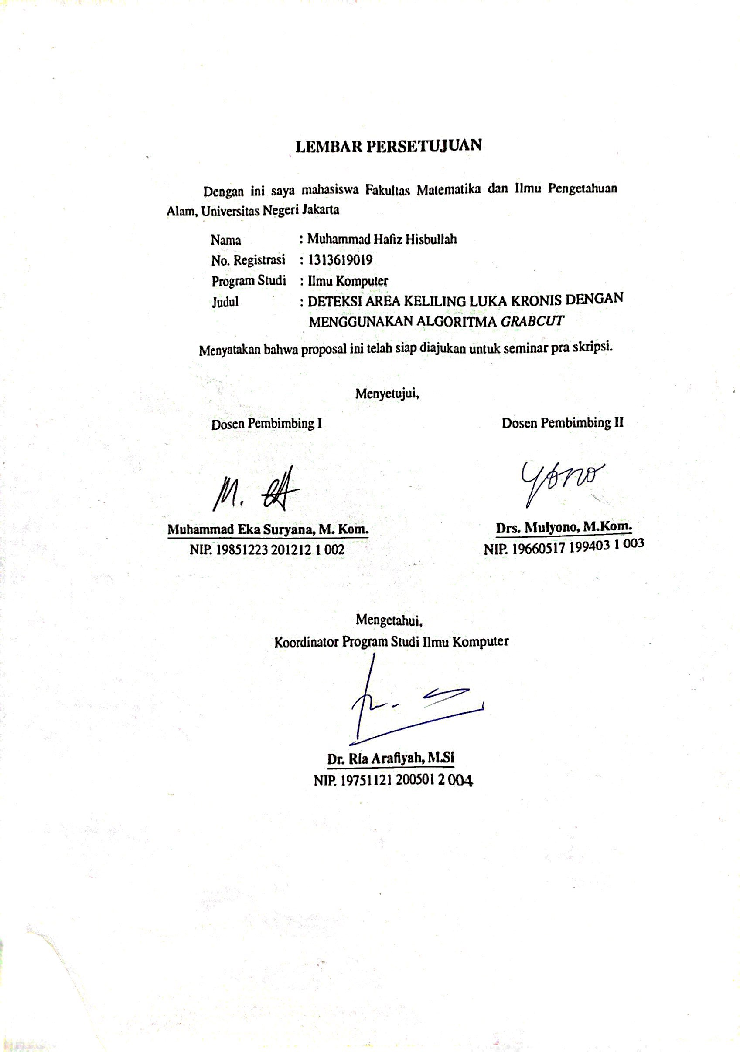
\includepdf[pages=-]{Lembar_Pengesahan.pdf}

% \chapter*{\centering{\large{LEMBAR PERSETUJUAN}}}
% \thispagestyle{empty} {\bf }Dengan ini saya mahasiswa Fakultas
% Matematika dan Ilmu Pengetahuan Alam, Universitas Negeri Jakarta

% \vskip3mm

% \begin{tabular}{ll}
%   Nama & : Muhammad Hafiz Hisbullah \\
%   No. Registrasi & : 1313619019 \\
%   Program Studi & : Ilmu Komputer \\
%   Judul & :  DETEKSI AREA KELILING LUKA KRONIS DENGAN \\ & \hspace{0.2cm} MENGGUNAKAN ALGORITMA \emph{GRABCUT}\\
% \end{tabular}

% \vskip3mm

% \noindent \hskip10mm Menyatakan bahwa proposal ini telah siap diajukan untuk seminar pra skripsi.
% %\begin{center}
% %Menyatakan bahwa skripsi ini telah siap diajukan untuk sidang skripsi.
% %\end{center}



% \begin{center}
% \vskip3mm

% Menyetujui,

% \vskip3mm
% \begin{spacing}{1.25}

% \begin{tabular}{ccc}
%   \hskip-2mm Dosen Pembimbing I & \qquad \qquad \qquad \qquad \qquad & \hskip-6mm Dosen Pembimbing II \\
%    &  &  \\
%    &  &  \\
%    &  &  \\
%    &  &  \\
%   \hskip-2mm \underline{\textbf{Muhammad Eka Suryana, M. Kom.}} &  & \hskip-6mm \underline{\textbf{Drs. Mulyono, M.Kom.}} \\
%   \hskip-2mm NIP. 19851223 201212 1 002 &  & \hskip-6mm NIP. 19660517 199403 1 003	 \\
% \end{tabular}
% \end{spacing}
% \end{center}
% \vskip3mm
% \begin{center}
% Mengetahui, \\
% Koordinator Program Studi Ilmu Komputer
% \end{center}
% \begin{spacing}{1.25}
% { \ }
% \\
% \\
% { \ }\begin{center}
% \underline{\textbf{Dr. Ria Arafiyah, M.Si}} \\
% {NIP. 19751121 200501 2 004}
% \end{center}
% \end{spacing} 
  